\chapter{System Description}

The system was largely built through previous experiments and consists of 3D-printed parts, a stepper motor, a camera, two metallic rods, a timing belt, and various mechanical components (see figure \ref{fig:overview_cart_pole_experiment})
\begin{figure}[htbp]
    \centering
    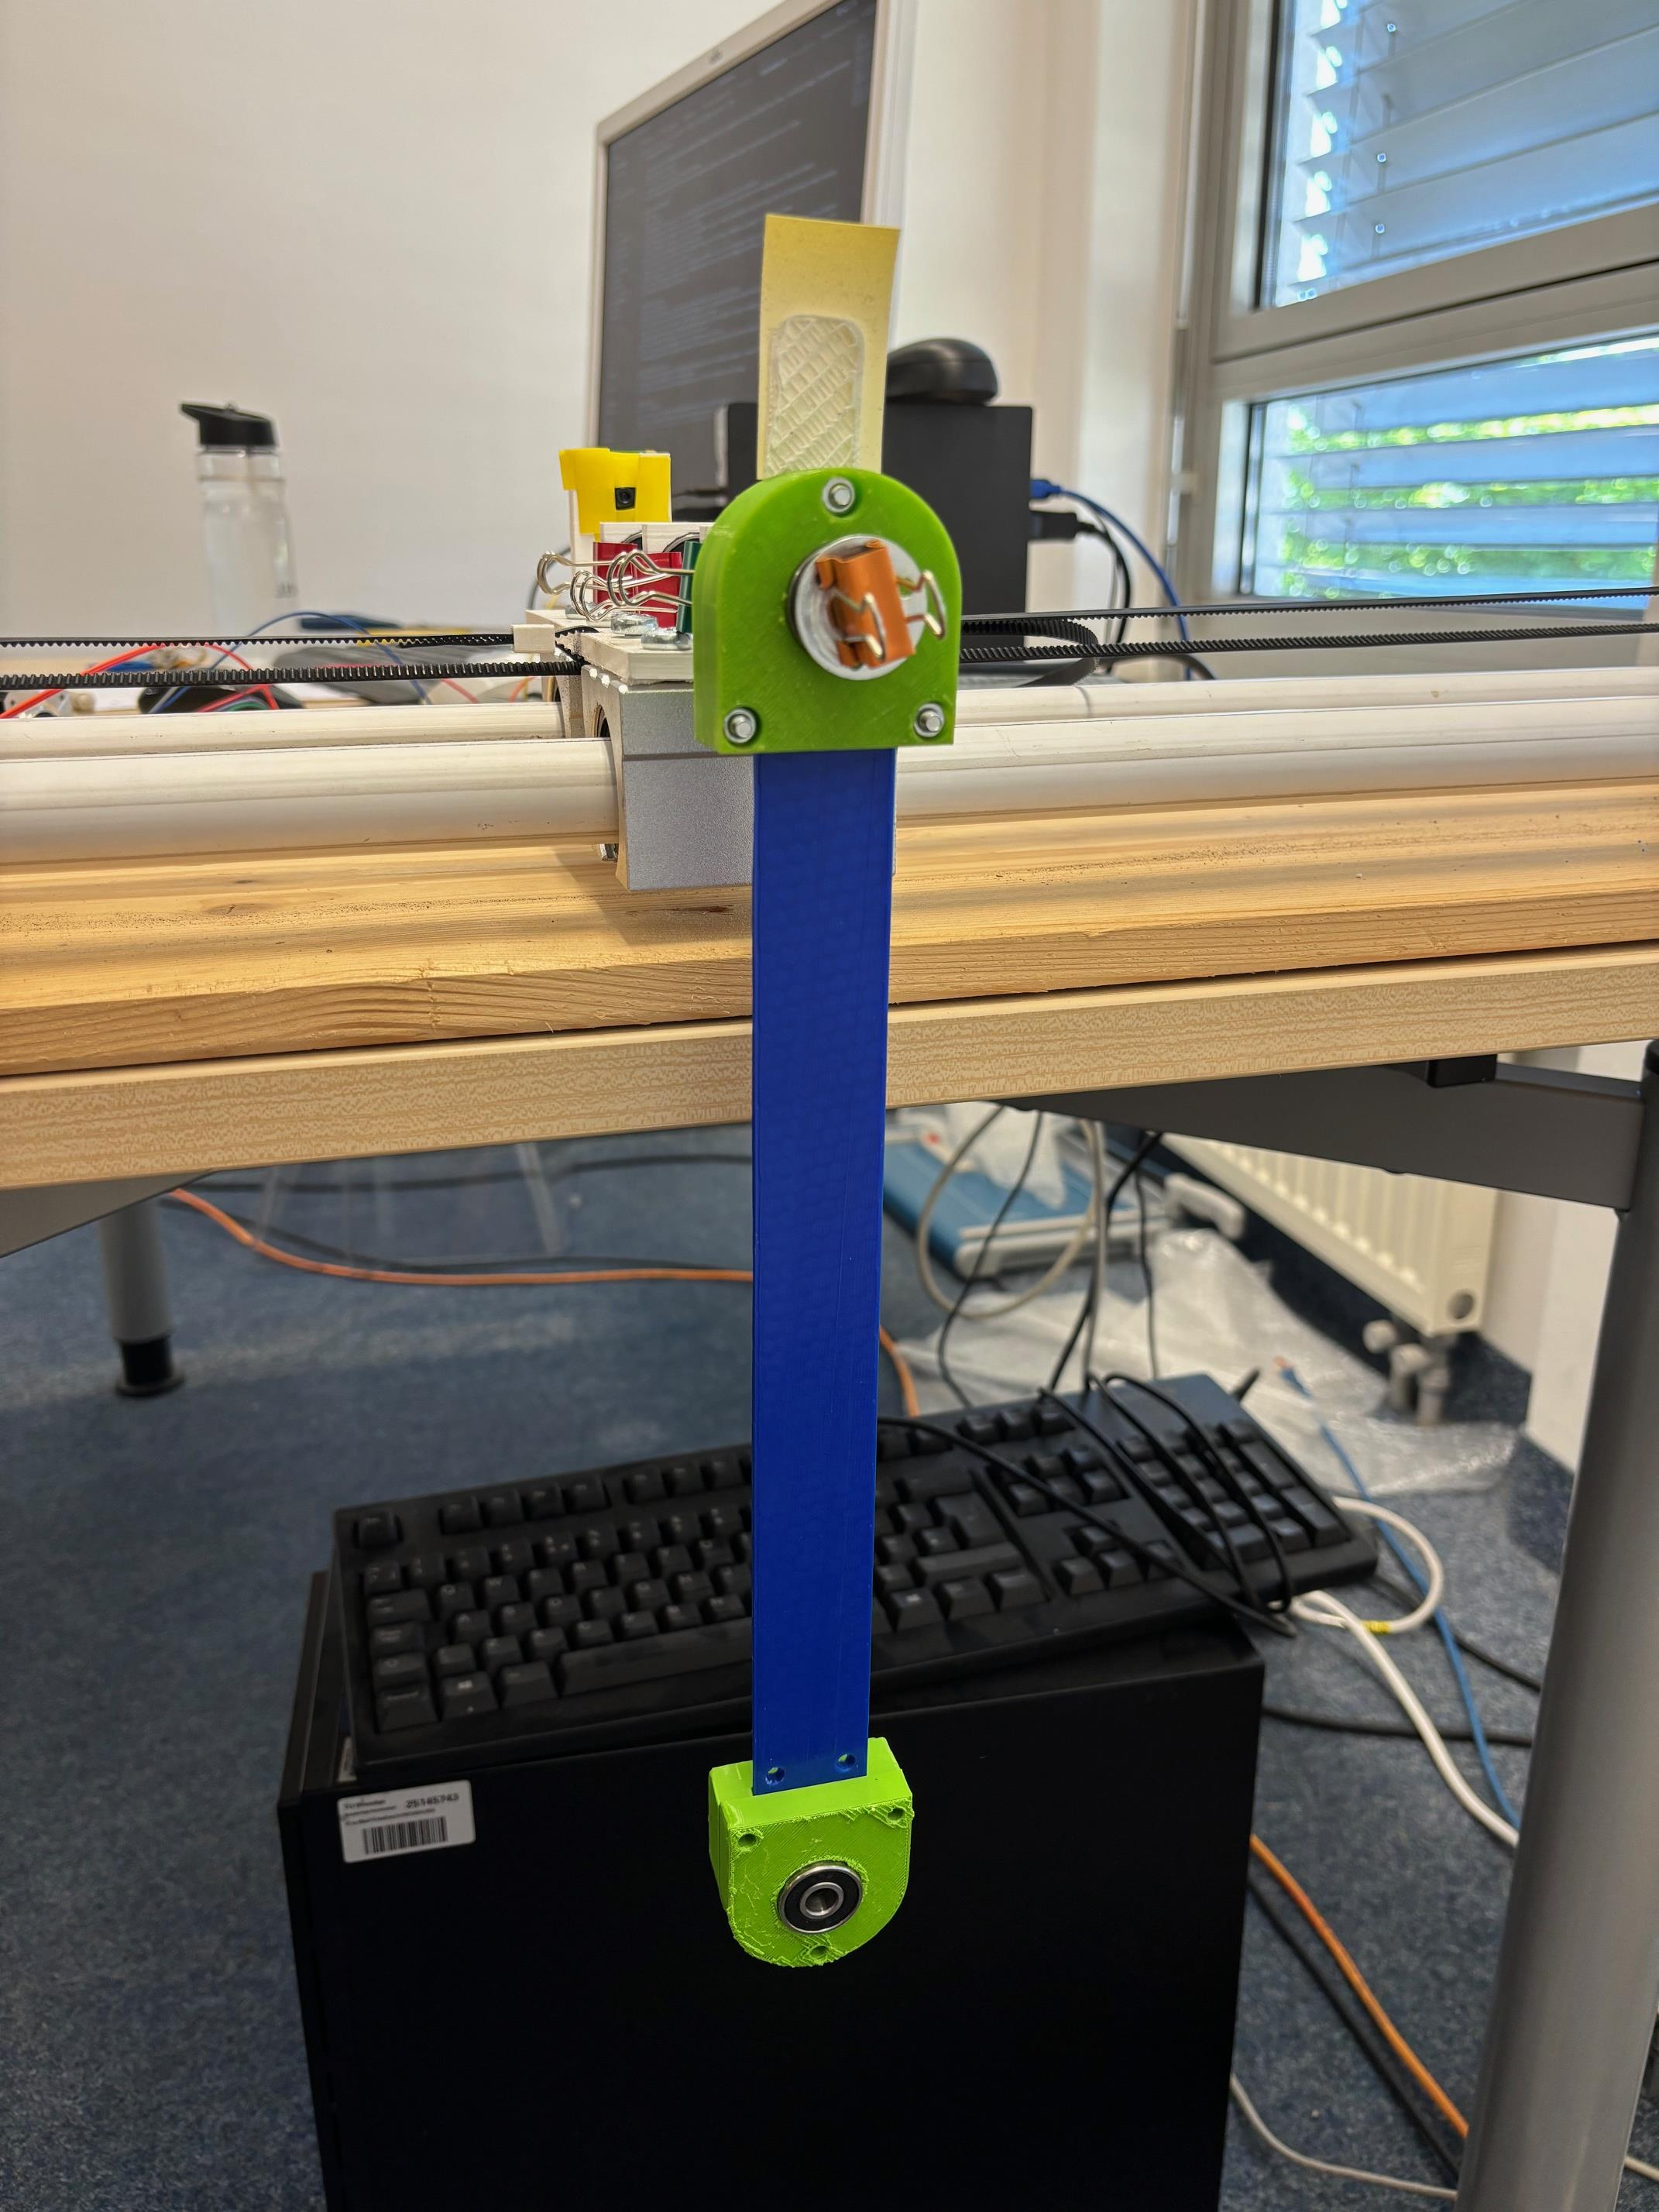
\includegraphics[width=0.4\textwidth]{img/front.jpg}
    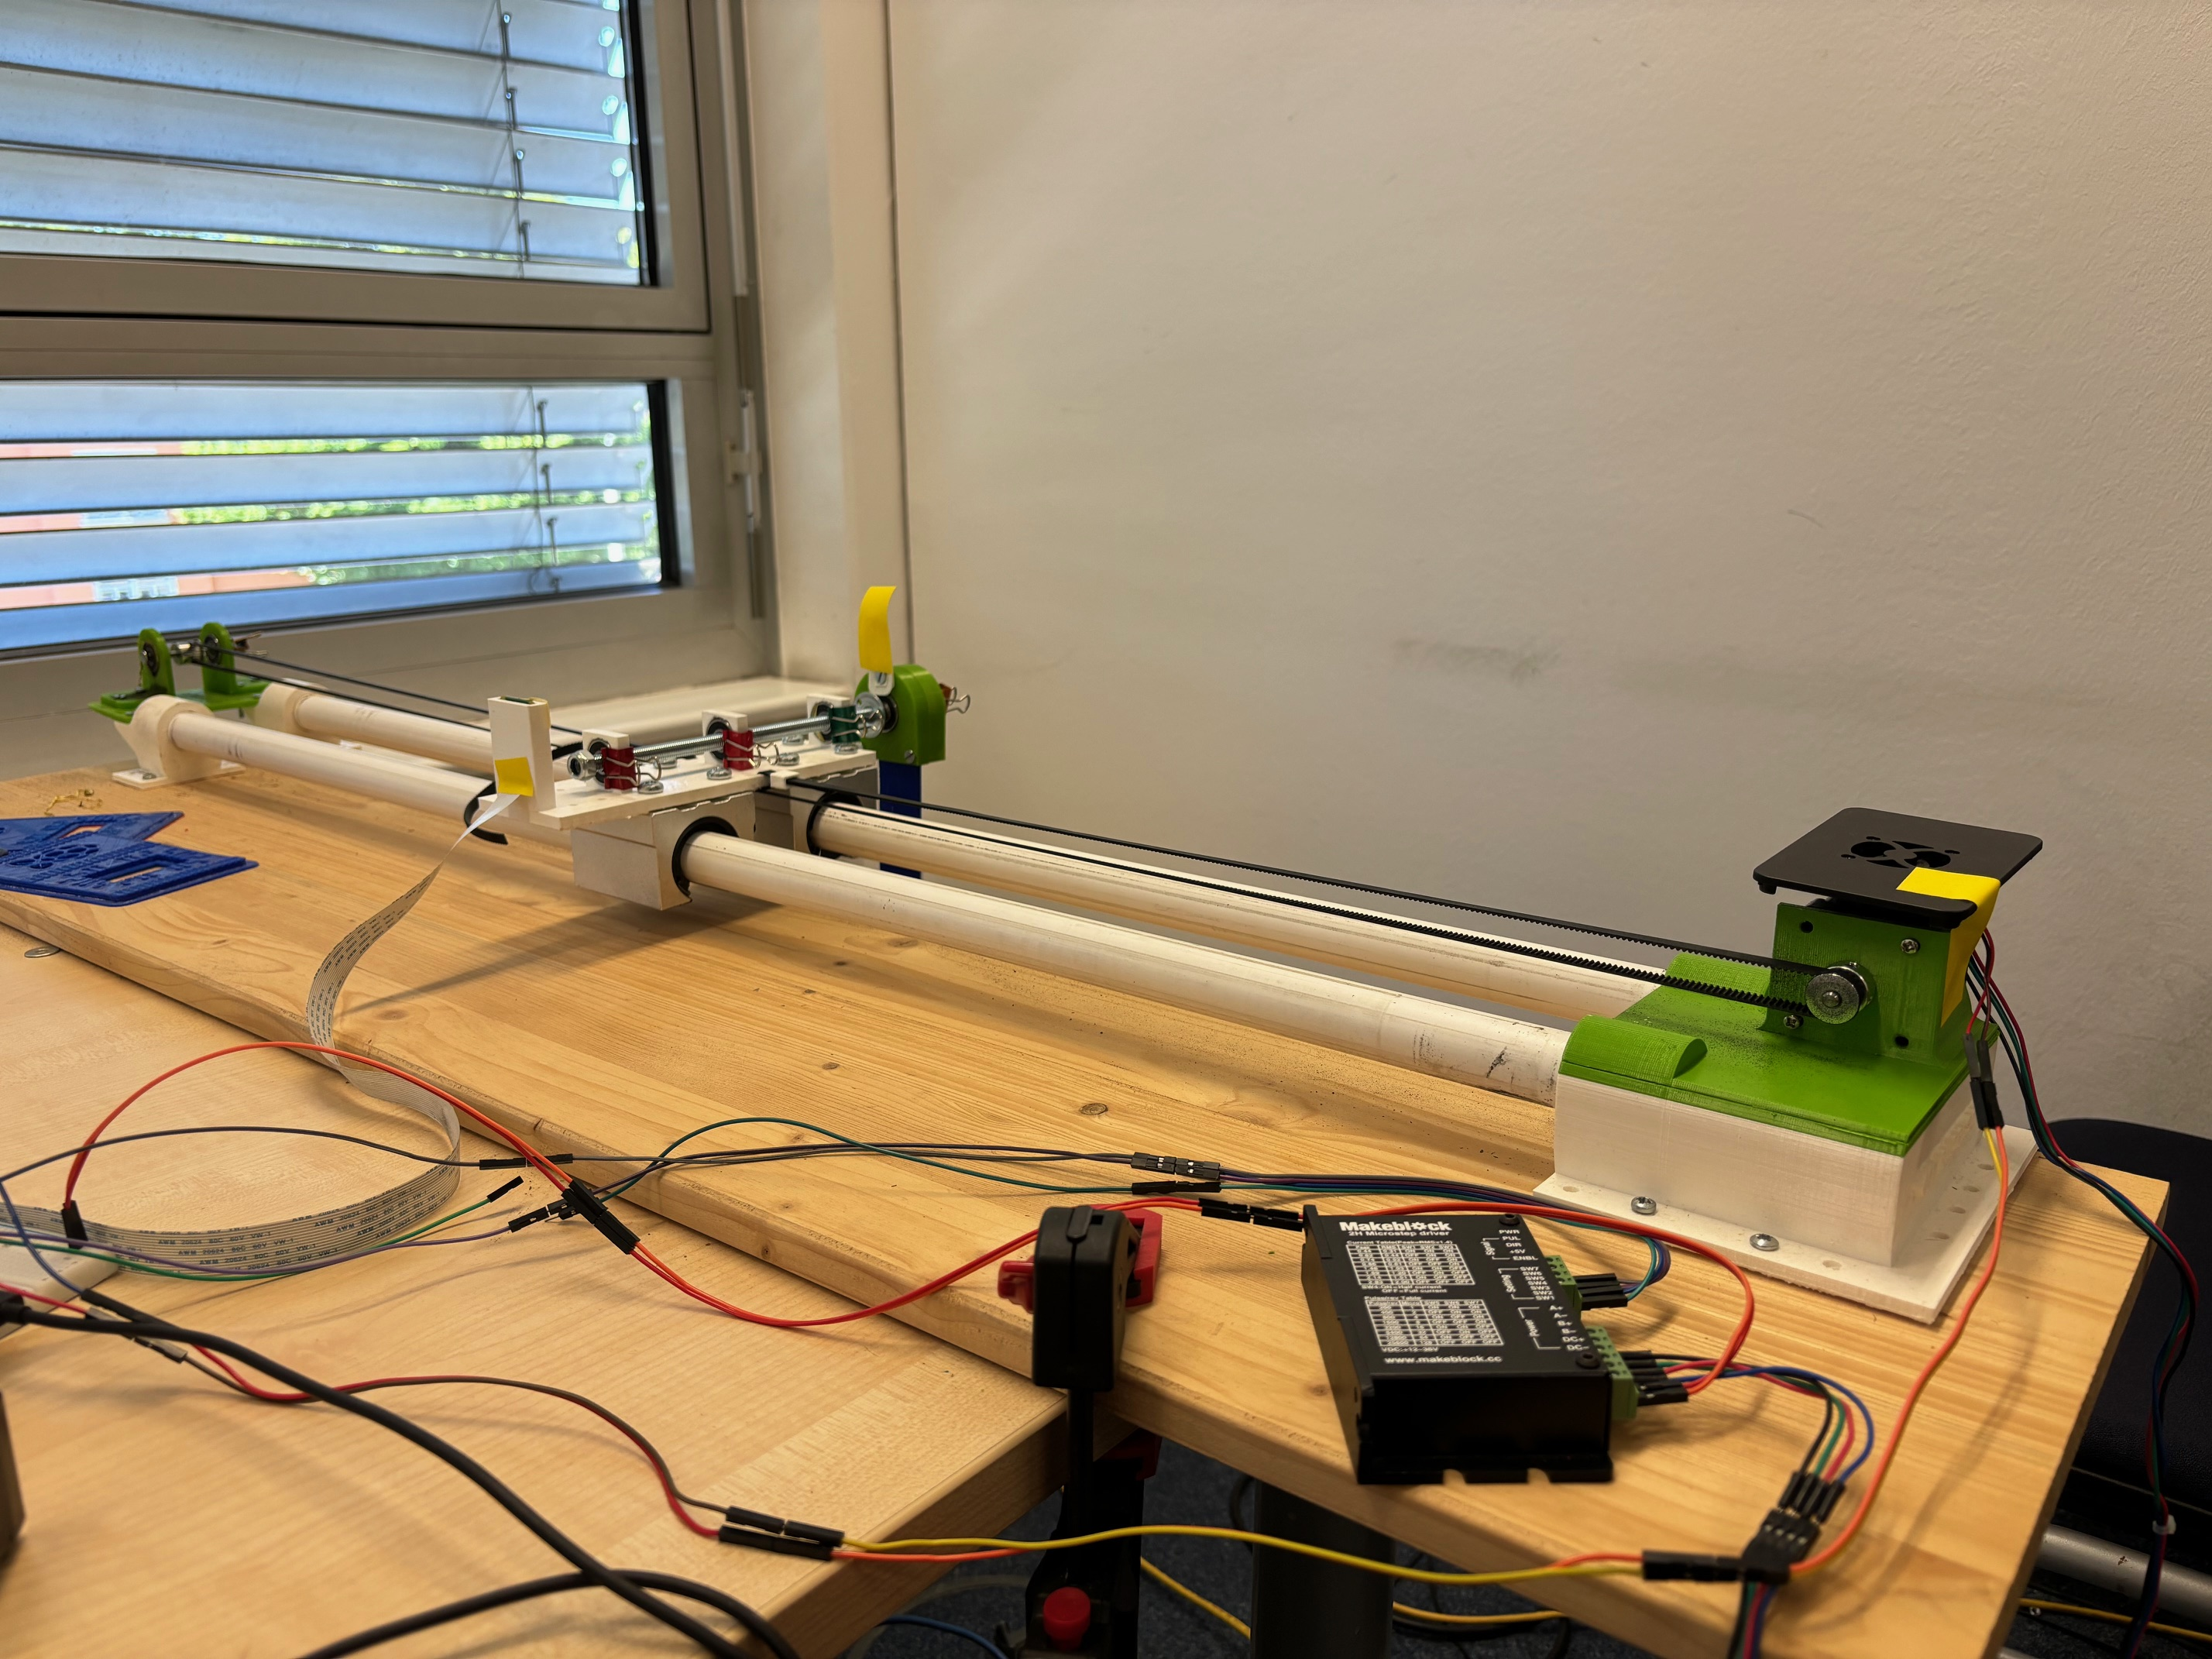
\includegraphics[width=0.4\textwidth]{img/back.jpg}
    \caption{Overview over Cart-Pole experiment with 3D printed parts}
    \label{fig:overview_cart_pole_experiment}
\end{figure}
Adjustments were made during the course of the experiments. Some of the moving parts shifted over time, necessitating the use of clamps to fix these parts in place (\ref{fig:clamps})
\begin{figure}[htbp]
    \centering
    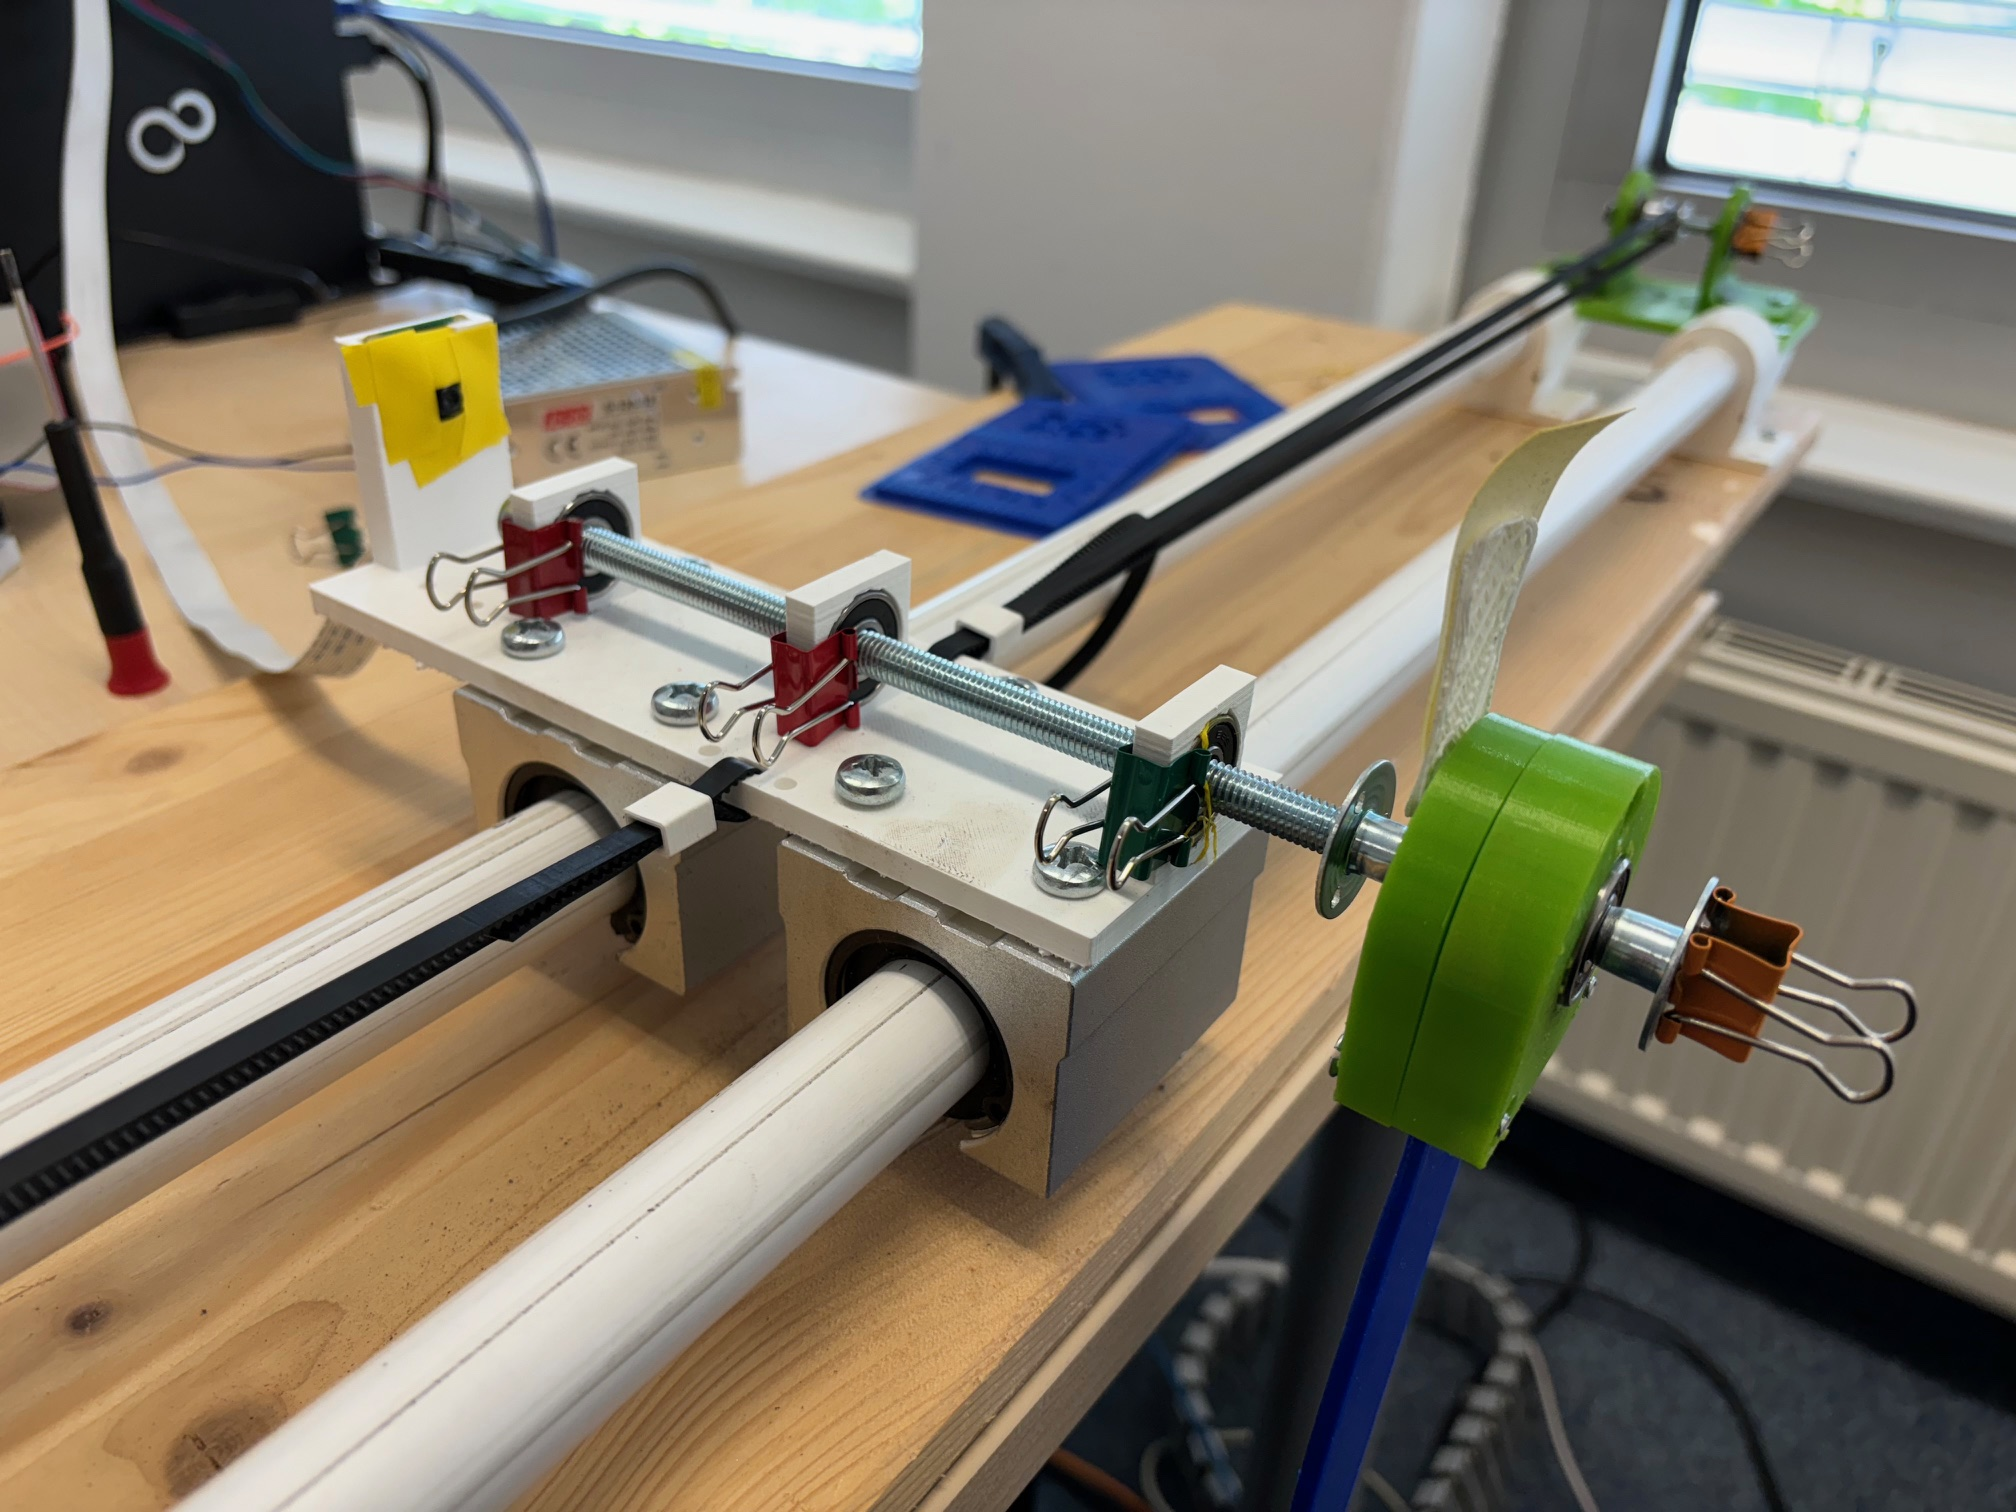
\includegraphics[width=0.8\textwidth]{img/clamps.jpg}
    \caption{Clamps to fixate moving parts}
    \label{fig:clamps}
\end{figure}

\section{Hardware Components}
\subsection{Cart}
\begin{figure}[htbp]
    \centering
    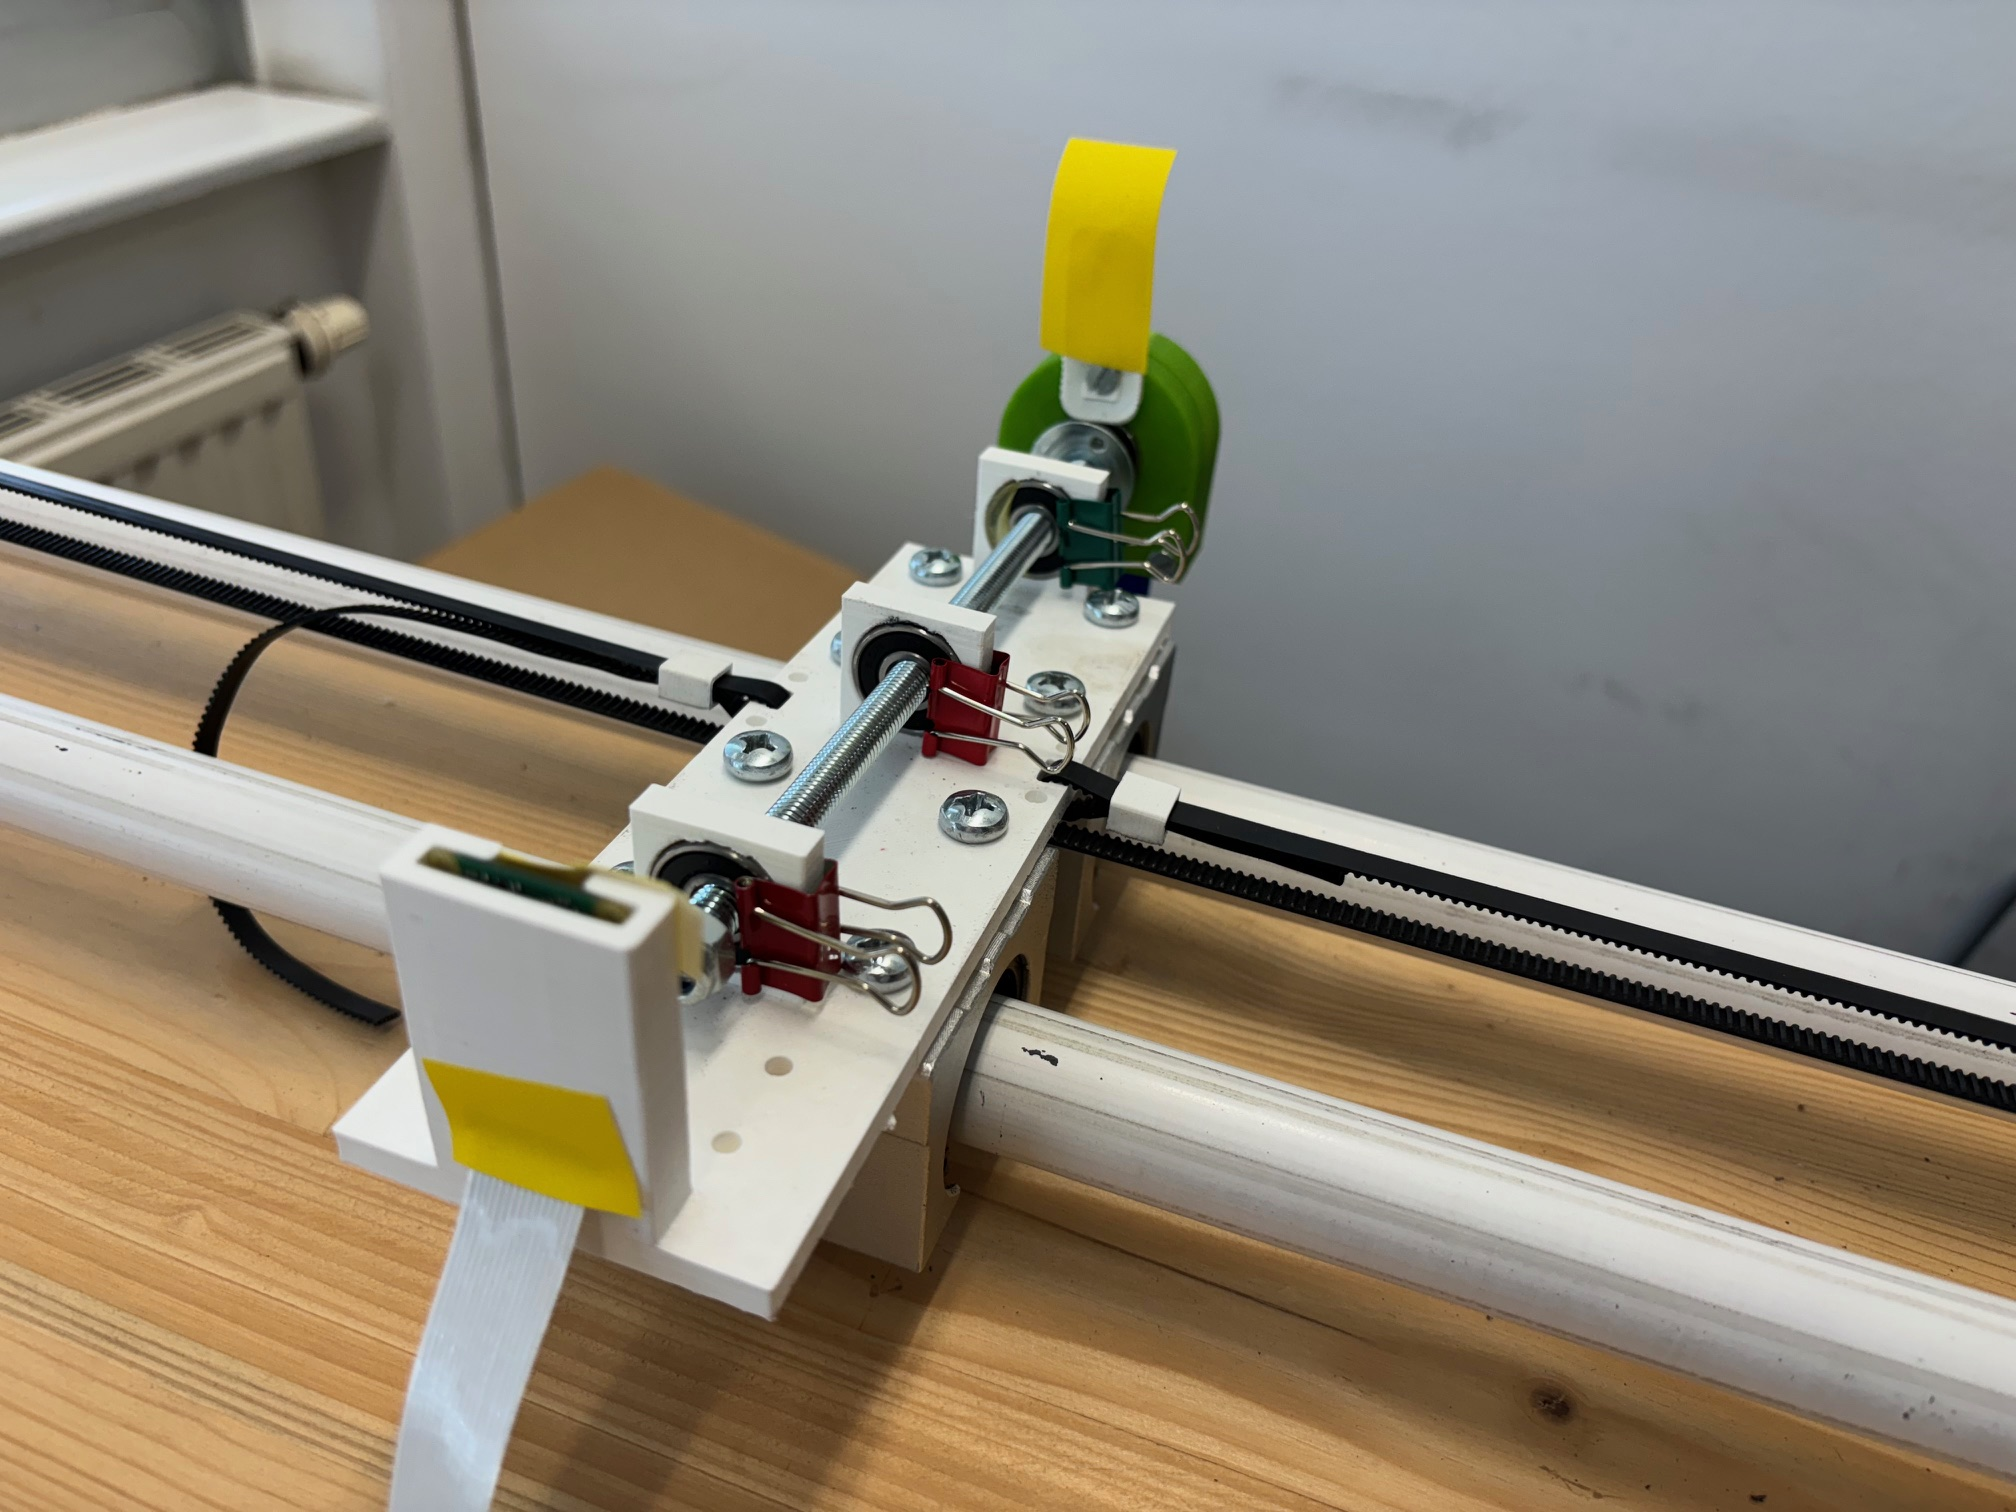
\includegraphics[width=0.8\textwidth]{img/cart.jpg}
    \caption{Cart from 3D printed parts with camera. Clamps are used to fixate moving parts.}
    \label{fig:cart}
\end{figure}
\begin{figure}[htbp]
    \centering
    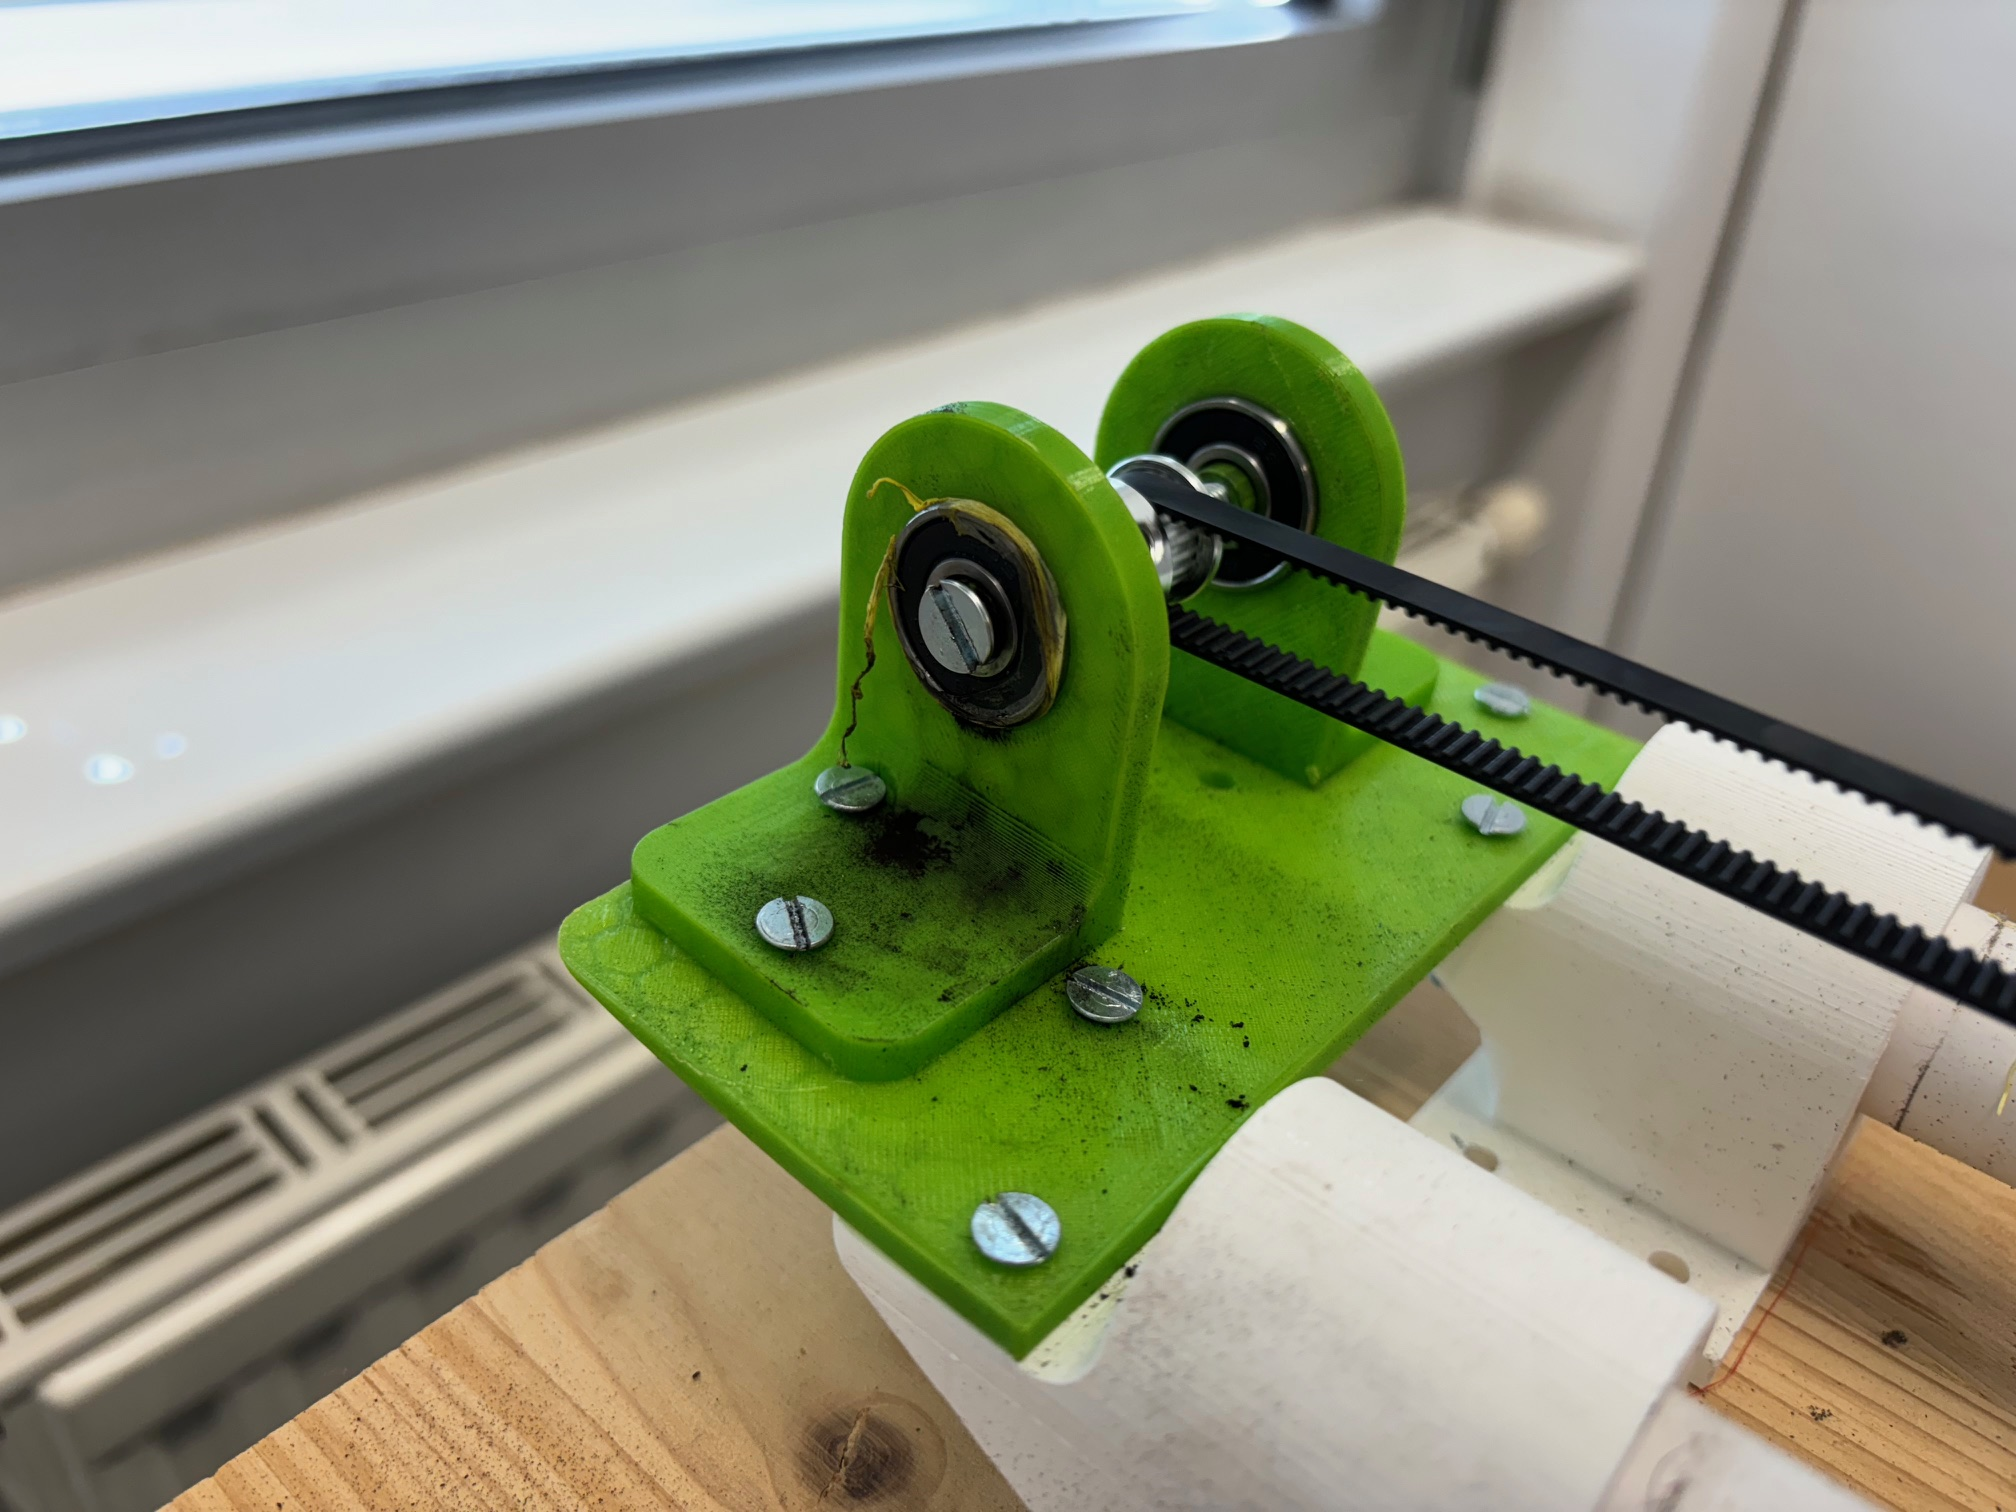
\includegraphics[width=0.8\textwidth]{img/deflection_pulley.jpg}
    \caption{Deflection pulley for the belt}
    \label{fig:deflection_pulley}
\end{figure}

The cart system is mounted on a wooden board with two supports spaced 95 cm apart, which hold the metal rods on which the cart (Figure \ref{fig:cart}) moves. One support has a deflection pulley in the form of a gear to guide the timing belt, while the other support mounts the stepper motor (Figure \ref{fig:deflection_pulley}). The timing belt must be very tight; otherwise, it slips, preventing the cart from moving.

There are several mounts for a threaded rod from which the pendulum hangs. The pendulum is 3D-printed and consists of five parts that fit together: one broad blue rod and four parts around the rod, two of which connect the pendulum to the thread, and two add extra weight at the end of the pendulum. A piece of plastic with yellow tape is also attached to the pendulum to enable the camera to recognize the pendulum's position.

The pendulum is 35 cm long and weighs 128 g. Although the cart-pole experiment ideally requires a smooth surface for the cart to move on, attempts to achieve this with rollers on the metal rods were insufficient. The surface was not smooth enough, requiring relatively more force to move the cart, complicating the experiments. However, according to Escobar et al. (\citeyear{manrique_escobar_parametric_2020}), this is not a significant problem, as the cart-pole experiment can also be solved with friction.

\subsection{Stepper Motor}
\begin{figure}[htbp]
    \centering
    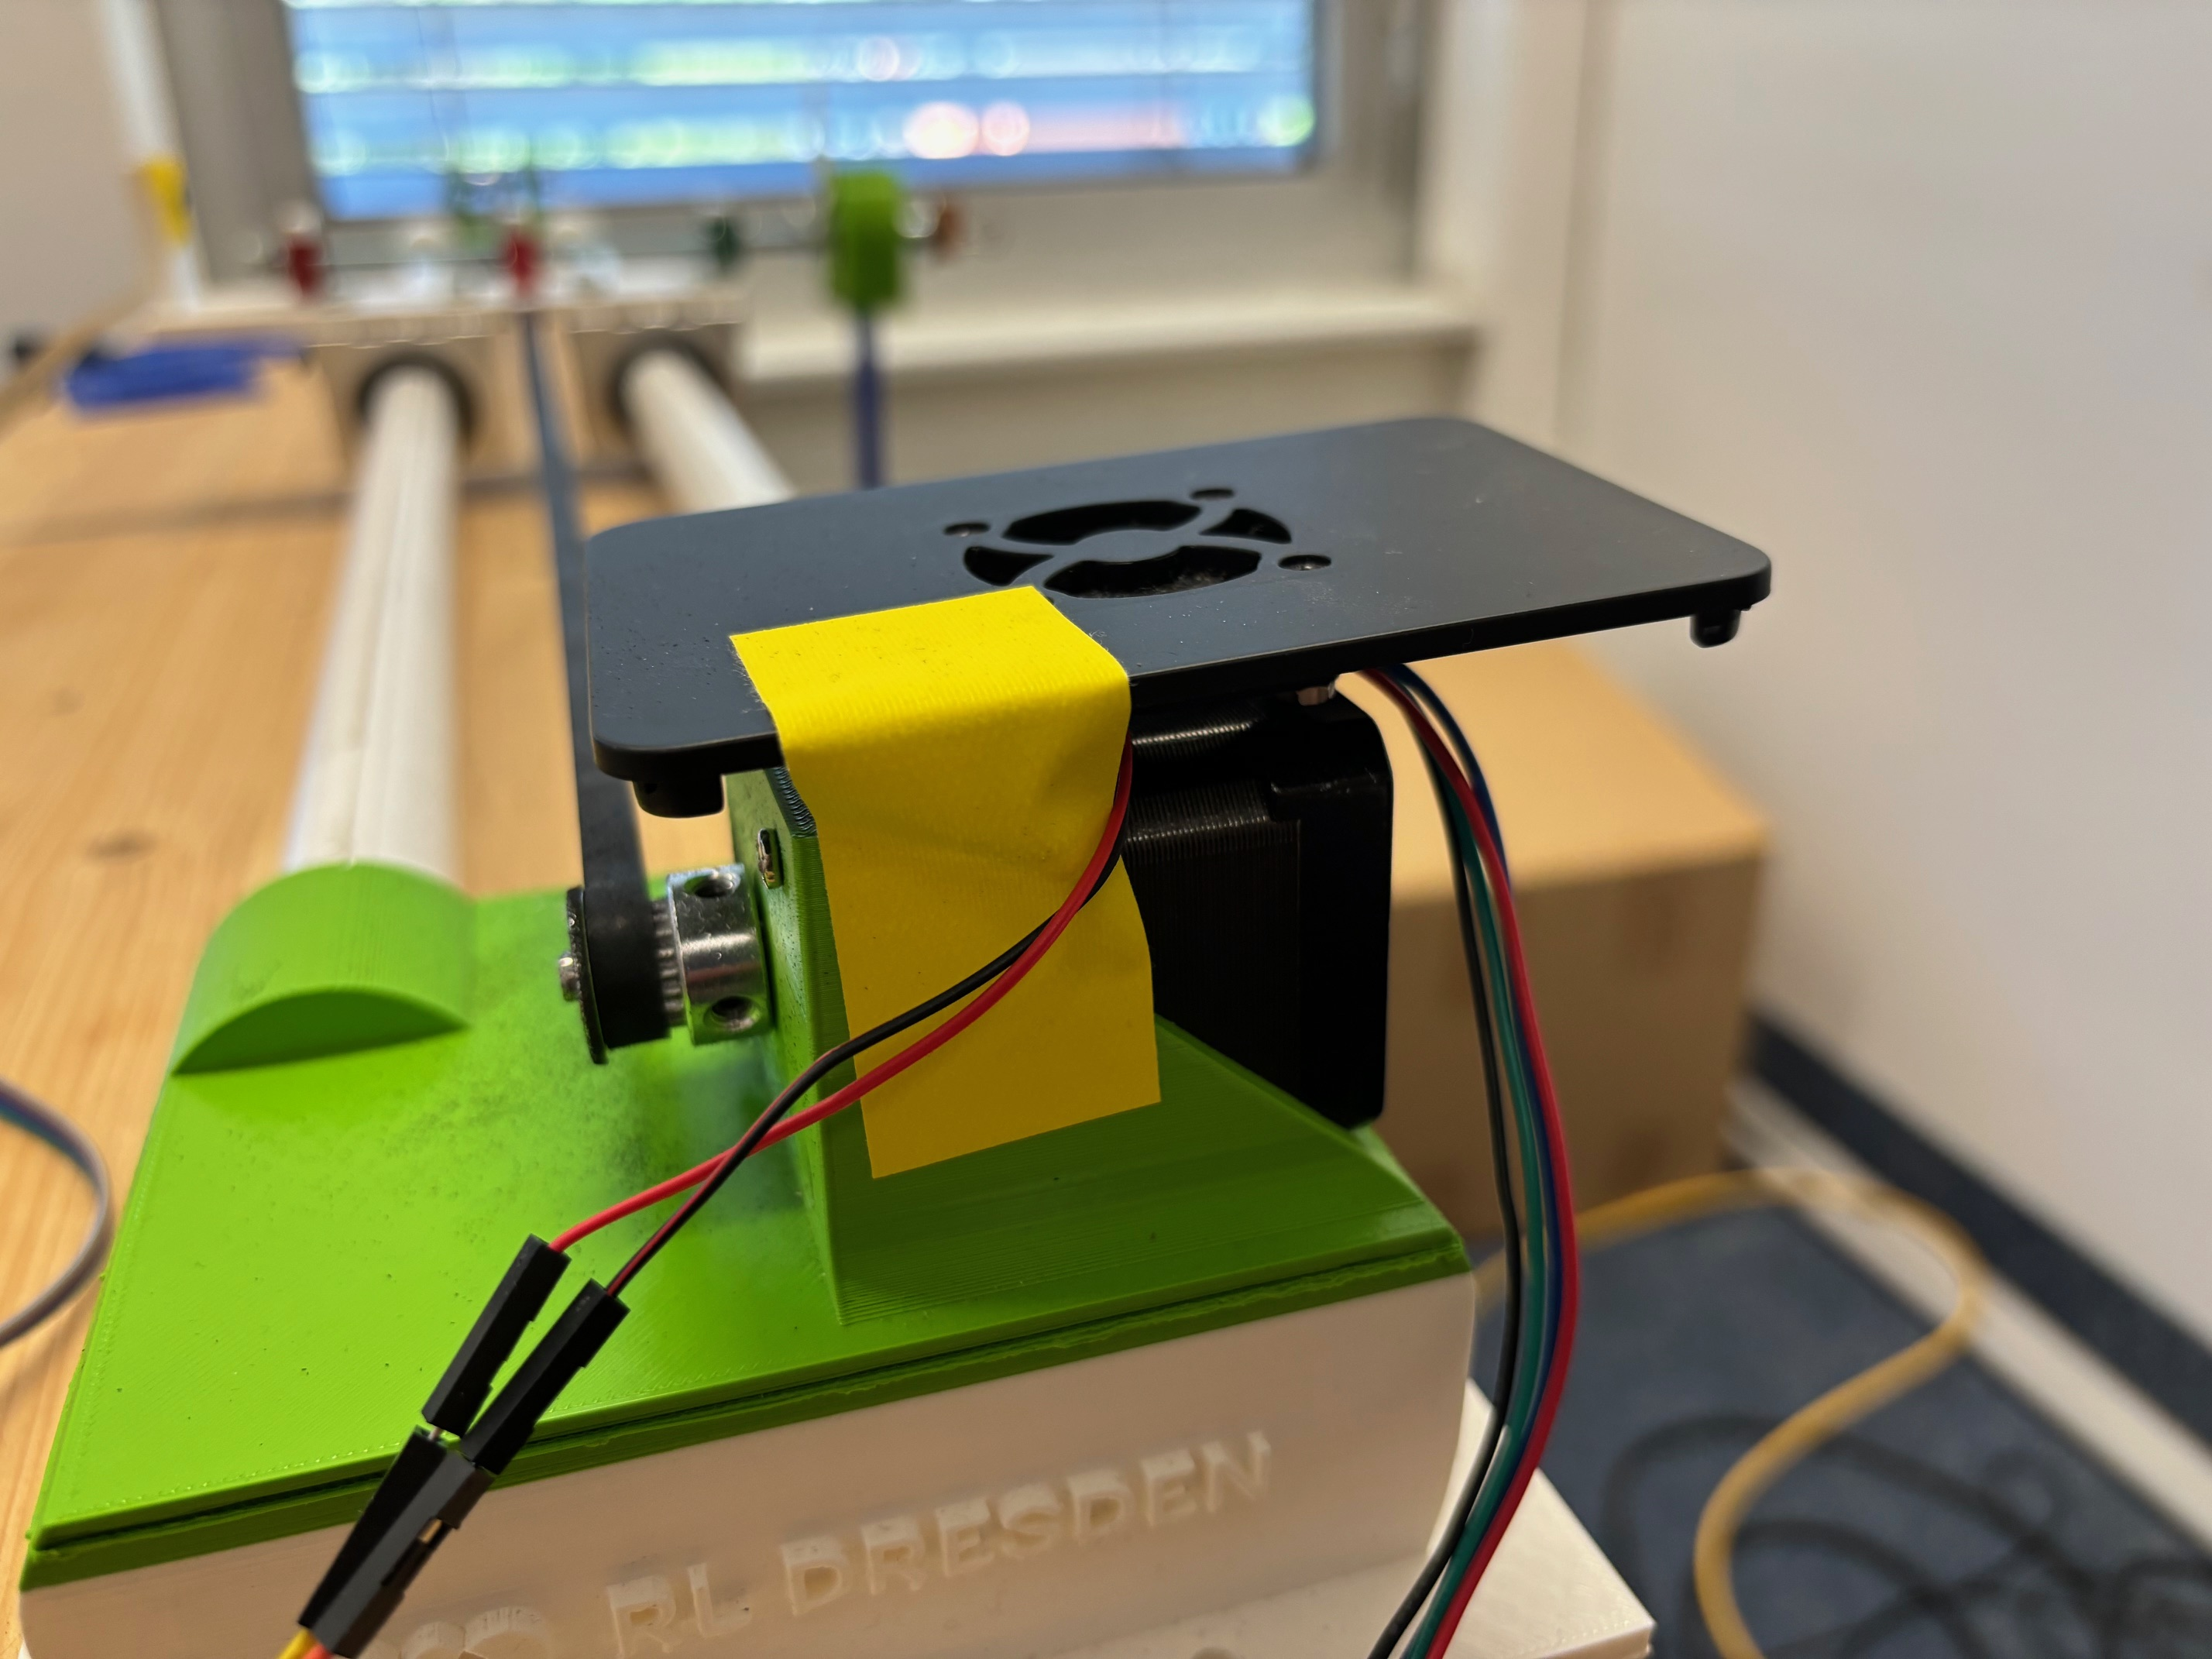
\includegraphics[width=0.8\textwidth]{img/stepper_motor.jpg}
    \caption{Stepper Motor for the Cart}
    \label{fig:stepper_motor}
\end{figure}
The stepper motor rotates a gear on which the timing belt is mounted, thereby moving the cart (Figure \ref{fig:stepper_motor}). During various experiments, different current levels were tested for the stepper motor. As the motor became hot, a fan was mounted. The fan is of the same type used for cooling a Raspberry Pi and operates at 3.3V.

Different stepper motors were tested throughout the experiments, all of the NEMA 17 type. One motor was labeled MOT-AN-S-060-005-042-L-A-AAAA from Igus, and two motors were labeled 17HS19-2004S1 from StepperOnline, one of which proved to be inaccurate. The Igus motor can handle a current of 1.8A, while the other motors can handle 2A.

The current was adjusted during the experiments to achieve the best performance without overheating the motor.

\subsection{Stepper Motor Control}
All motors were controlled using a Makeblock 2H Microstep Driver, which is connected to an Arduino. The Arduino is connected to a Raspberry Pi via Micro-USB. All stepper motors were operated with a step angle resolution of 1.8$^\circ$ (12800 steps per revolution).

\subsection{Camera}
\begin{figure}[htbp]
    \centering
    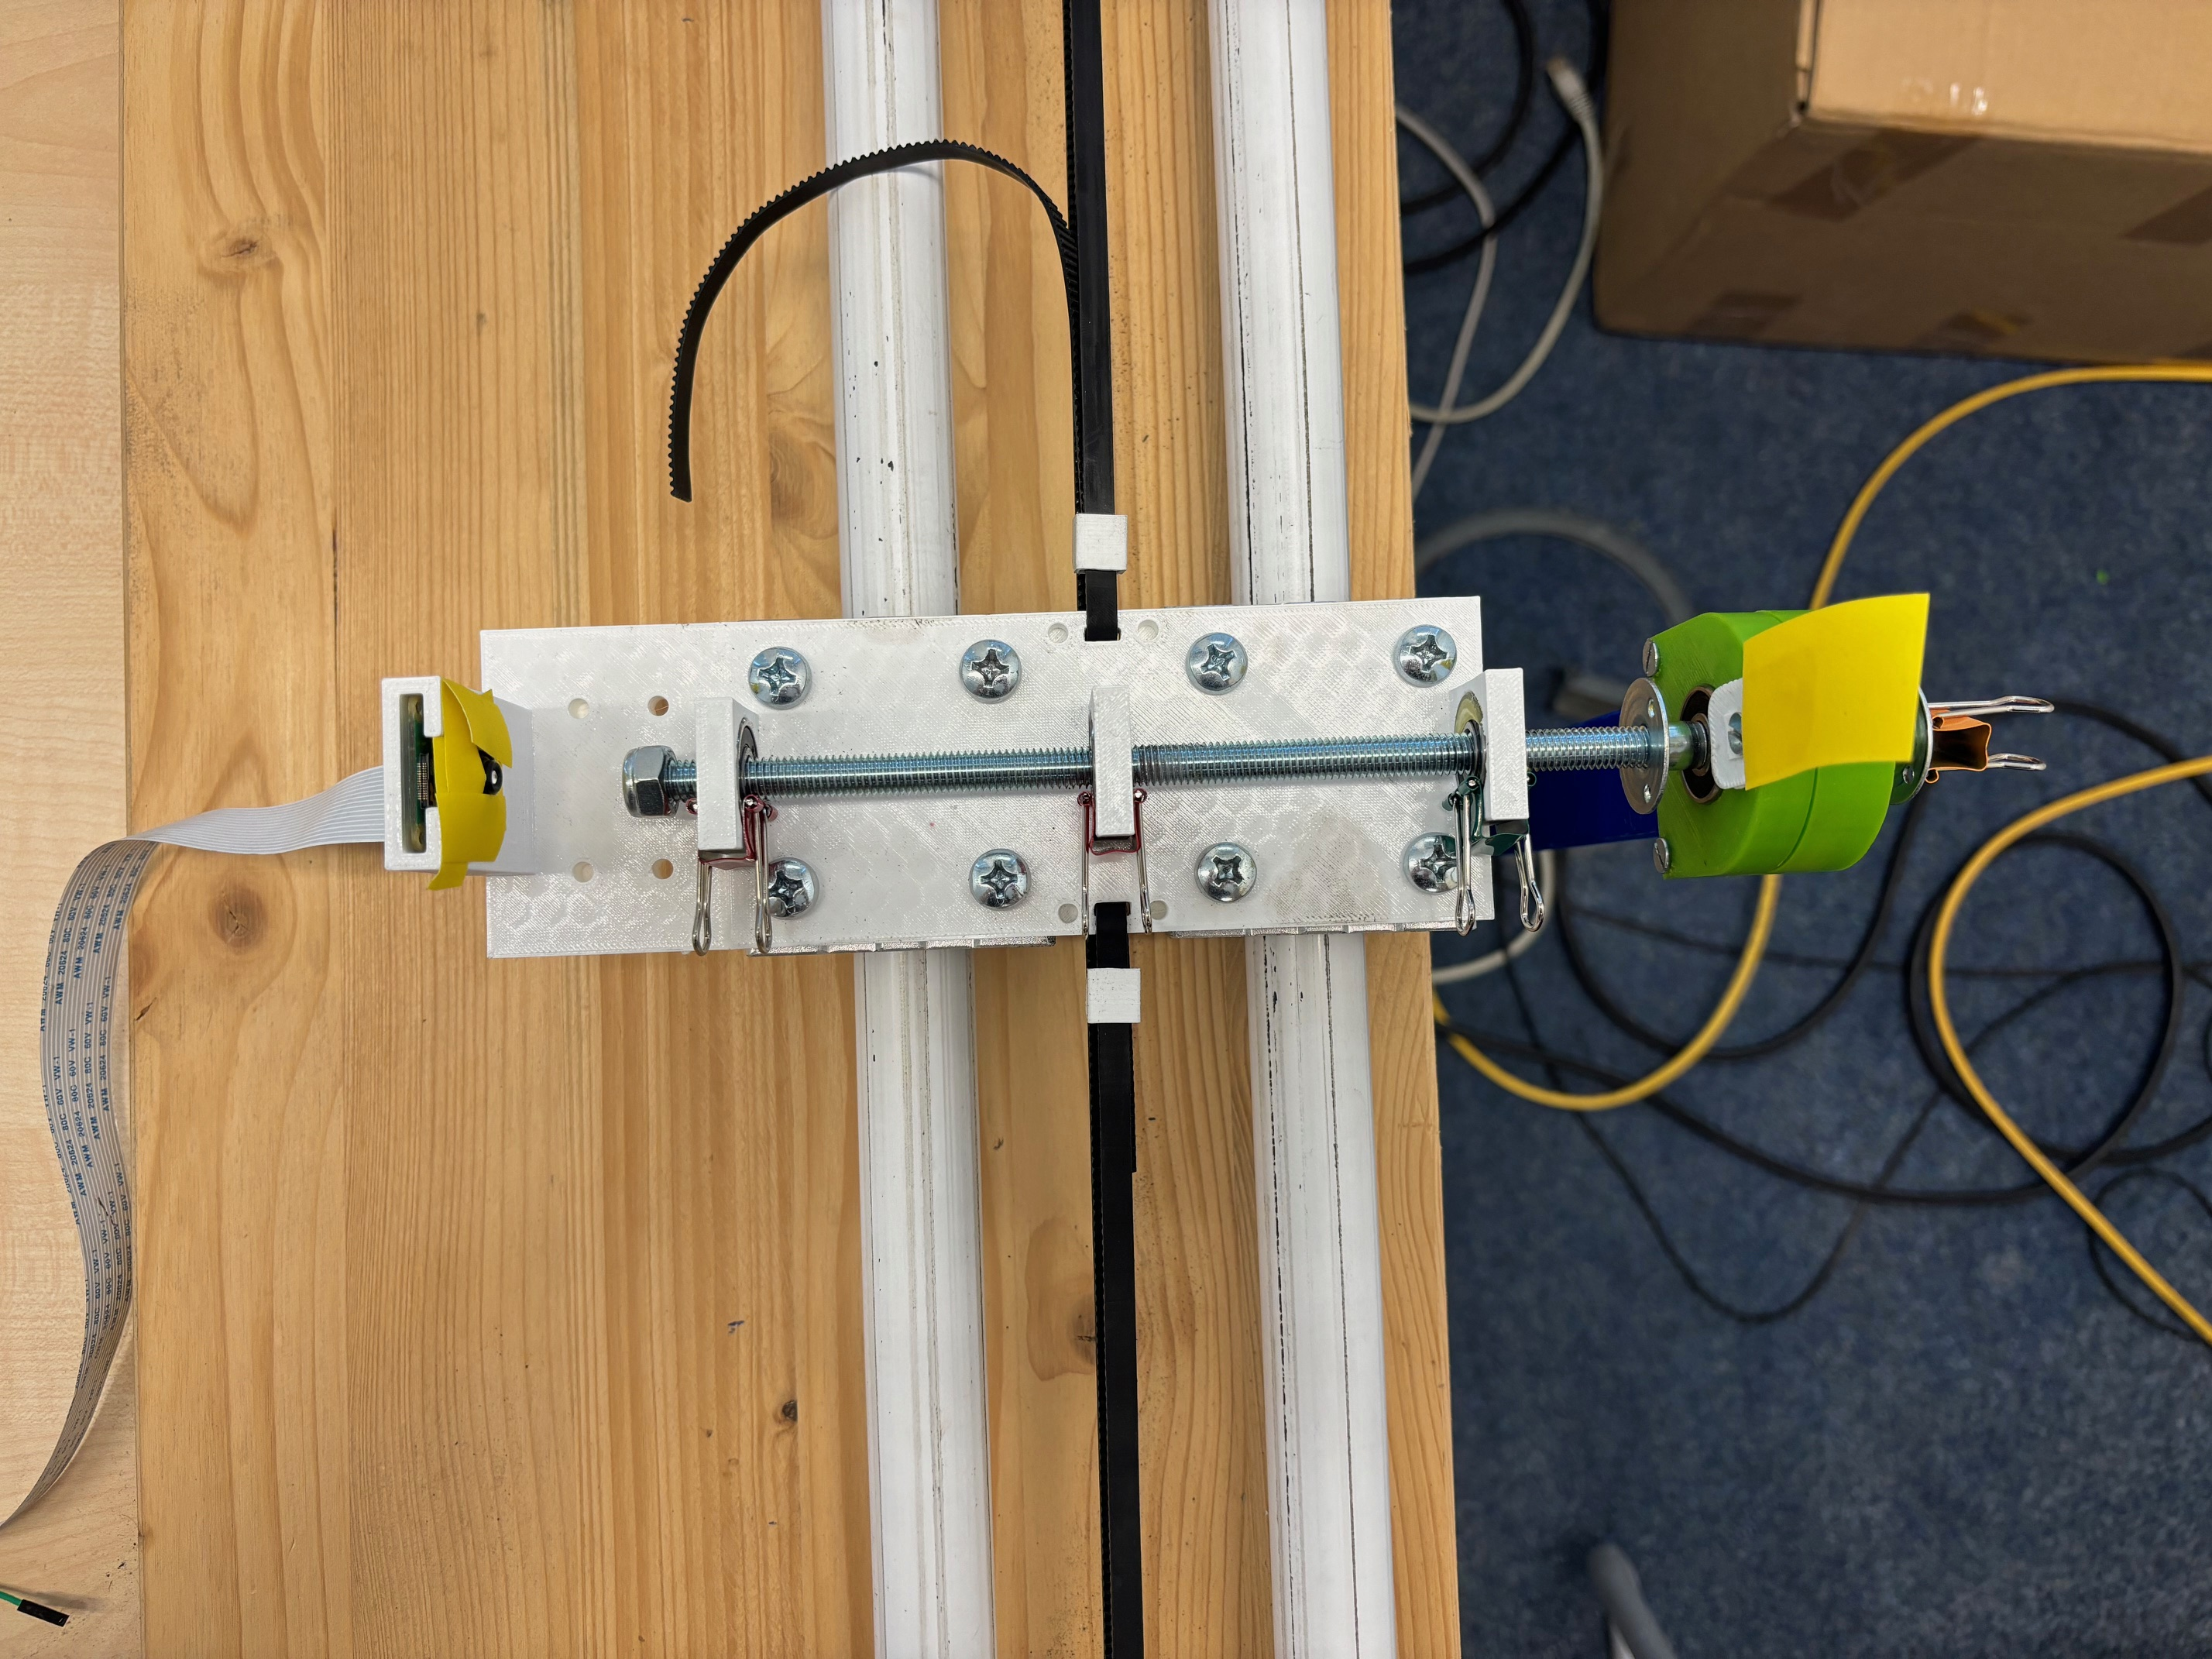
\includegraphics[width=0.8\textwidth]{img/camera.jpg}
    \caption{Camera to detect the angle of the pendulum}
    \label{fig:camera}
\end{figure}
The camera used is a Picam, mounted in a 3D-printed housing attached to the cart (Figure \ref{fig:camera}). The camera is connected to a Raspberry Pi, which processes the images captured by the camera. It is crucial that the position of the camera remains fixed; otherwise, the angles of the pendulum detected will not be accurate.

To improve image processing speed and maintain consistent focus, the autofocus feature of the camera was disabled. Tape was used to secure the camera and ensure it stays in a fixed position.

\section{Software Architecture}
\subsection{Reinforcement Learning Agent}
A custom environment based on OpenAI Gym was developed to simulate the cart-pole environment. The most significant modification involved overriding the step function to convert selected actions into messages sent to the Arduino to move the cart. The algorithm used is Proximal Policy Optimization (PPO), implemented using Stable Baselines 3. Image processing from the camera is handled by a separate script, which runs independently of the reinforcement learning agent to determine the angles of the pendulum. Angles start at 0 in the upper position and range up to 180 degrees in the lower position; on the left side of the pendulum from 0 to 180 degrees, and on the right side from 0 to -180 degrees. The angles and other information are sent to the reinforcement learning agent using ZeroMQ's implementation of a TCP socket. This setup allows for better utilization of the Raspberry Pi's four cores (one core for the RL agent, one core for image processing), more frequent image captures, more accurate determination of angular velocity through more measurements, and reduced decision delay for the RL agent, as images no longer need processing before action selection.

\subsection{Control Algorithms}
Communication between the Raspberry Pi and the Arduino occurs over USB as a serial connection. A custom protocol is used where messages are transmitted as strings. These strings follow the format \textit{<letter,number>}, where letters represent the type of message and numbers represent the values, see table \ref{tab:types_of_messages}.
\begin{table}
    \caption{Types of messages for the Arduino}
    \label{tab:types_of_messages}
    \begin{tabular}{|c|c|}
        \hline
        Type & Description \\
        \hline
        v & Set the speed in steps per second \\
        a & Set the acceleration in steps per second$^2$ \\
        m & Move the stepper motor to a certain position \\
        r & Move the stepper motor relative to its current position \\
        h & Set the current position as home position. Value is always 0 \\
        s & Set the steps per revolution \\
        p & Get the current position. Value is always 0 \\
        \hline
    \end{tabular}
    \end{table}
The Arduino always knows the current position by counting the steps performed and automatically stops the motor when the cart reaches the end of the rods. Therefore, it is necessary to set the home position in the middle of the track section the cart is supposed to travel to ensure it always stops when reaching the end. The maximum number of revolutions of the stepper motor before the cart reaches the end of the rods was determined to be nine. The Raspberry Pi sends messages to the Arduino to move the cart, and due to the system's asynchrony, the Raspberry Pi can perform other calculations in the meantime to determine the next action of the reinforcement learning agent while the cart is moving. The Arduino continues to move the cart at the specified speed until it receives a new message or the cart reaches the end of the rod.

Additionally, a function was implemented to detect whether the office is empty to avoid disturbing employees with the noise produced by the moving cart. Whether the office is empty currently depends only on the time. It is assumed that the office is occupied from 8:30 AM to 6:30 PM from Monday to Friday. Outside these hours, it is assumed the office is empty, and the cart can move without disturbing anyone. This check is performed each time the RL agent is reset (calling the reset function of the Gym environment). If the office is not empty, the system waits 10 minutes before checking again.